\section{8-Queens problem}

\begin{figure}[H]
    \centering
    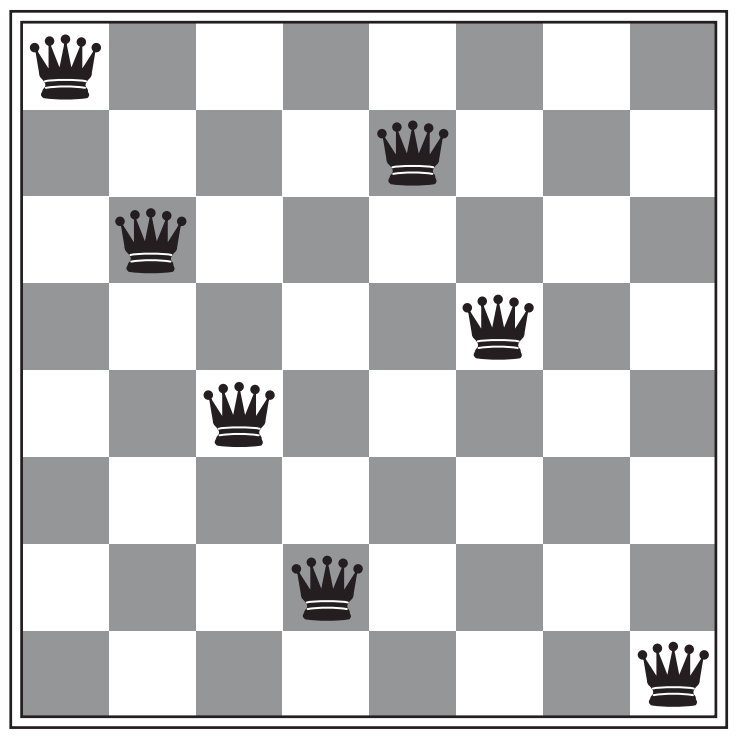
\includegraphics[
        width=\linewidth,
        height=5cm,
        keepaspectratio,
    ]{images/artificial-intelligence/examples/8-queens-problem.png}
    \caption{Almost a solution to the 8-queens problem. the queen in the rightmost column is attacked by the queen at the top left.}
\end{figure}


\begin{enumerate}
    \item The goal of the 8-queens problem is to place eight queens on a chessboard such that no queen attacks any other.
    (A queen attacks any piece in the same row, column or diagonal.)
    \hfill \cite{ai/book/Artificial-Intelligence-A-Modern-Approach/Russell-Norvig}

    \item
    \hfill \cite{ai/book/Artificial-Intelligence-A-Modern-Approach/Russell-Norvig}
\end{enumerate}


\subsection{As a Problem Solving Agent}

\begin{enumerate}
    \item \textbf{States}: Any arrangement of 0 to 8 queens on the board is a state.
    \hfill \cite{ai/book/Artificial-Intelligence-A-Modern-Approach/Russell-Norvig}

    \item \textbf{Initial state}: No queens on the board.
    \hfill \cite{ai/book/Artificial-Intelligence-A-Modern-Approach/Russell-Norvig}

    \item \textbf{Actions}: Add a queen to any empty square.
    \hfill \cite{ai/book/Artificial-Intelligence-A-Modern-Approach/Russell-Norvig}

    \item \textbf{Transition model}: Returns the board with a queen added to the specified square.
    \hfill \cite{ai/book/Artificial-Intelligence-A-Modern-Approach/Russell-Norvig}

    \item \textbf{Goal test}: 8 queens are on the board, none attacked.
    \hfill \cite{ai/book/Artificial-Intelligence-A-Modern-Approach/Russell-Norvig}
\end{enumerate}



\subsection{As a Hill Clibing Agent}

\begin{figure}[H]
    \centering
    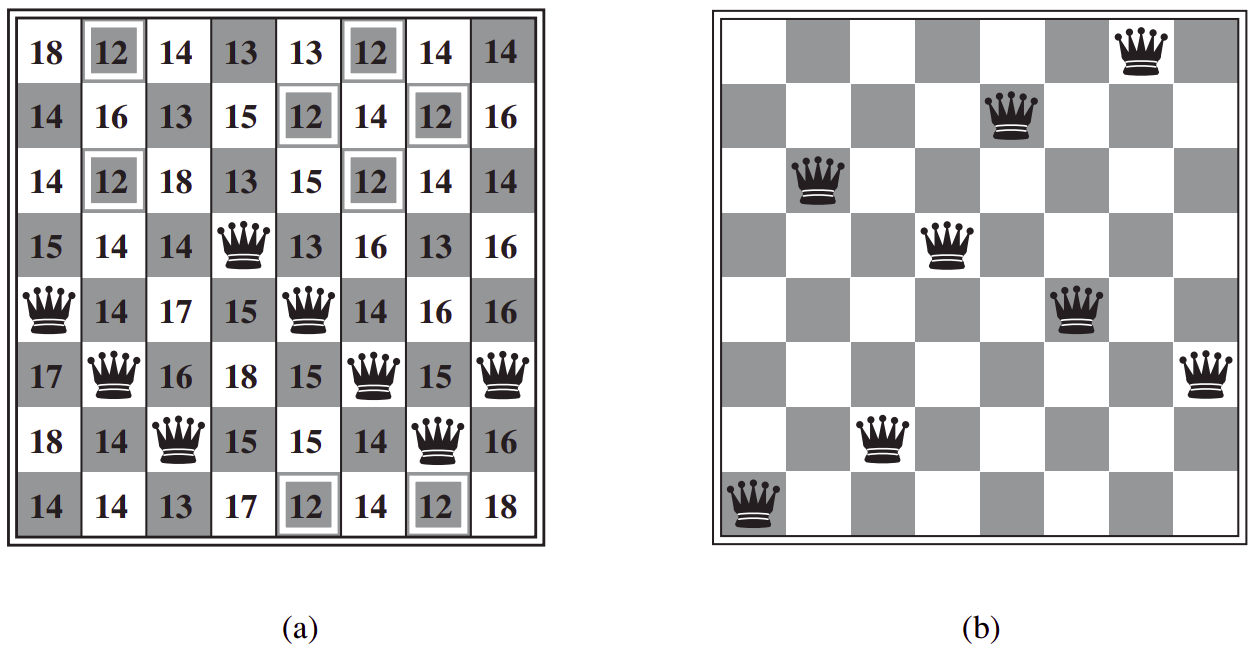
\includegraphics[
        width=\linewidth,
        height=5cm,
        keepaspectratio,
    ]{images/artificial-intelligence/examples/8-queens-hill-climbing.png}
    \caption{
        (a) An 8-queens state with heuristic cost estimate h = 17, showing the value of h for each possible successor obtained by moving a queen within its column. The best moves are marked.
        \hfill \cite{ai/book/Artificial-Intelligence-A-Modern-Approach/Russell-Norvig}
        \\
        (b) A local minimum in the 8-queens state space; the state has h = 1 but every successor has a higher cost.
        \hfill \cite{ai/book/Artificial-Intelligence-A-Modern-Approach/Russell-Norvig}
    }
\end{figure}

\vspace{0.5cm}

\begin{enumerate}
    \item each state has $8$ queens on the board, one per column
    \hfill \cite{ai/book/Artificial-Intelligence-A-Modern-Approach/Russell-Norvig}

    \item The successors of a state are all possible states generated by moving a single queen to another square in the same column (so each state has $8 \times 7 = 56$ successors).
    \hfill \cite{ai/book/Artificial-Intelligence-A-Modern-Approach/Russell-Norvig}

    \item The heuristic cost function $h$ is the number of pairs of queens that are attacking each other, either directly or indirectly.
    \hfill \cite{ai/book/Artificial-Intelligence-A-Modern-Approach/Russell-Norvig}

    \item The global minimum of this function is zero, which occurs only at perfect solutions.
    \hfill \cite{ai/book/Artificial-Intelligence-A-Modern-Approach/Russell-Norvig}
\end{enumerate}



\subsection{Using Genetic Algorithm}

\begin{figure}[H]
    \centering
    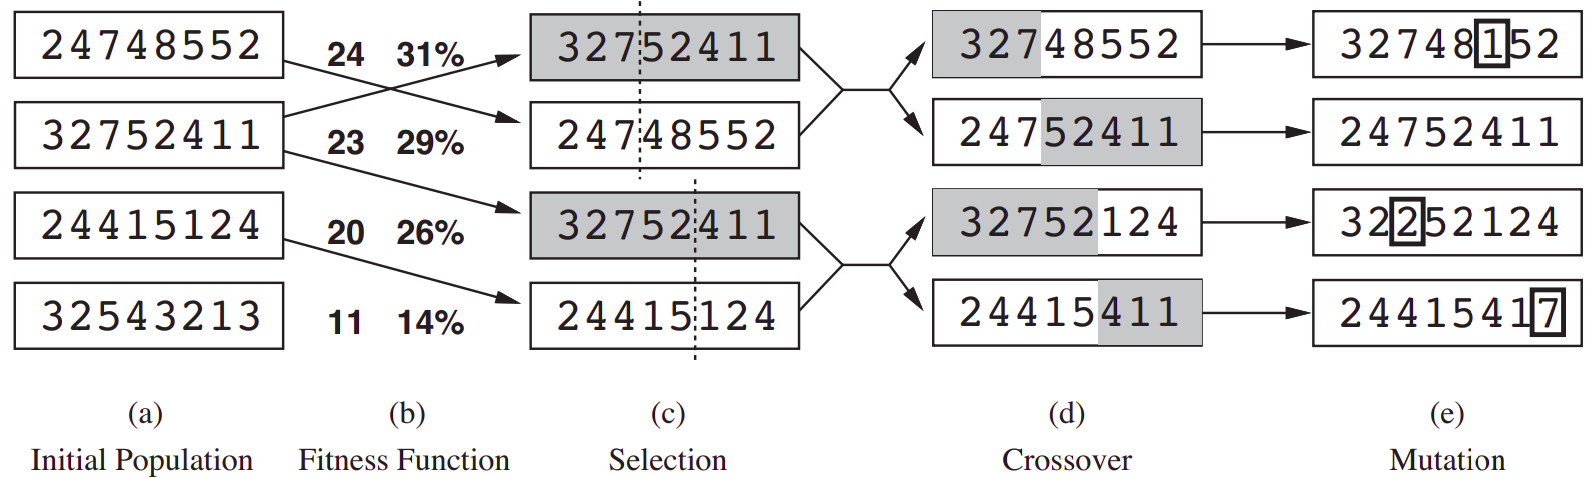
\includegraphics[
        width=\linewidth,
        height=4cm,
        keepaspectratio,
    ]{images/artificial-intelligence/examples/genetic-algo-8-queens-stages.png}
    \caption{
        The genetic algorithm, illustrated for digit strings representing 8-queens states.
        The initial population in (a) is ranked by the fitness function in (b), resulting in pairs for mating in (c). They produce offspring in (d), which are subject to mutation in (e).
        \cite{ai/book/Artificial-Intelligence-A-Modern-Approach/Russell-Norvig}
    }
\end{figure}


\begin{figure}[H]
    \centering
    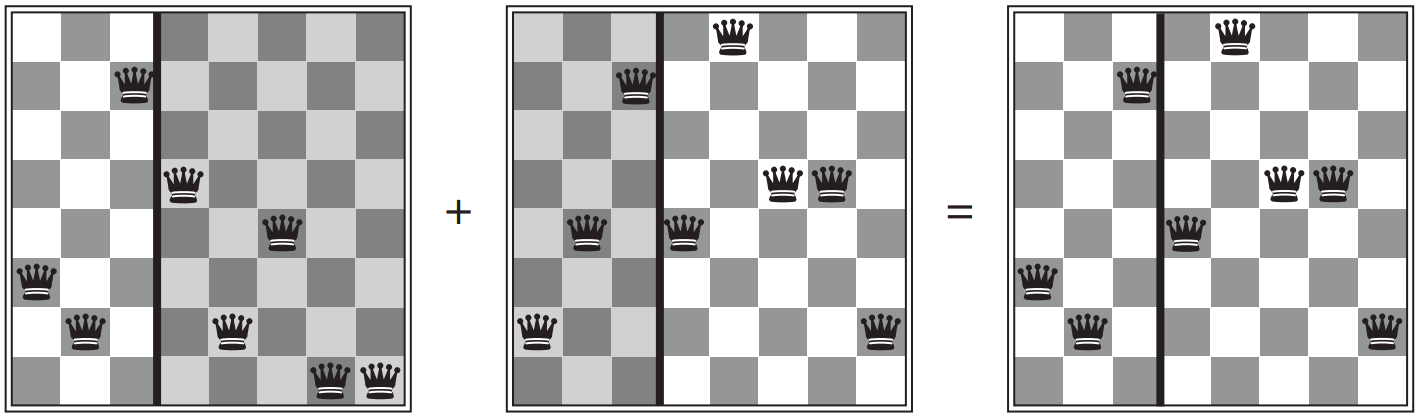
\includegraphics[
        width=\linewidth,
        height=4cm,
        keepaspectratio,
    ]{images/artificial-intelligence/examples/genetic-algo-8-queens.png}
    \caption{
        The 8-queens states corresponding to the first two parents (c) and the first offspring (d).
        The shaded columns are lost in the crossover step and the unshaded columns are retained.
        \cite{ai/book/Artificial-Intelligence-A-Modern-Approach/Russell-Norvig}
    }
    \label{fig:enter-label}
\end{figure}


\begin{enumerate}
    \item an $8$-queens state must specify the positions of $8$ queens, each in a column of $8$ squares, and so requires $8 \times log_2 8 = 24$ bits.
    Alternatively, the state could be represented as 8 digits, each in the range from $1$ to $8$.
    \hfill \cite{ai/book/Artificial-Intelligence-A-Modern-Approach/Russell-Norvig}
\end{enumerate}

















